\section{Kristallstrukturen} \label{kap:2}
Hier: ideale Kristalle, also unendliche Wiederholungen von identischen Strukturen (keine Oberfläche, Defekte, \dots)
\begin{itemize}
    \item Bekannte Atomsorte(n) und Bindungsart: wohldefinierte Gleichgewichtslängen.
    \item Gesamtenergie des Kristalls ist minimal, wenn alle Bausteine genau dieselbe Umgebung vorfinden
    \item \textbf{Struktur} Beschreibung als \textbf{Basis} (Strukturelement) + \textbf{Gitter} (Bauplan, Aneinanderreihung der Strukturelemente)
          \begin{itemize}
              \item Basis: 1 Atom (Au), 2 Atome (Diamant, Si, NaCl, GaAs), \dots, 13 Atome (YBa$_2$Cu$_3$O$_7$), \dots $>10^4$ Atome in Proteinkristallen
              \item Gitter: In 3D nur 14 Bravais-Gitter
          \end{itemize}
\end{itemize}

\subsection{Kristallgitter} \label{kap:2_1}
\textbf{Def.:} Unendlich große, regelmäßige, periodische Anordnung von Raumpunkten. Es sieht immer gleich aus, unabhängig von welchem Gitterpunkt aus es betrachtet wird.\\
Das Kristallgitter wird durch die \textbf{fundamentalen Gittervektoren} \textbf{a$_1$}, \textbf{a$_2$}, \textbf{a$_3$} aufgespannt, d.h. jeder Gitterpunkt durch $\textbf{R} = n_1 \textbf{a}_1 + n_2 \textbf{a}_2 +n_3 \textbf{a}_3$ ($n_1$, $n_2$, $n_3$ ganzzahlig) beschrieben. Die Länge der fundamentalen Gittervektoren definiert die sog. \textbf{Gitterkonstante}.\\
\textbf{Primitive Gittervektoren} erreichen (bei vorgegebenem Ursprung) alle Gitterpunkte.\\
Die (primitiven) GV \textbf{a$_1$}, \textbf{a$_2$}, \textbf{a$_3$}, spannen ein Parallelepiped auf. Dieses stellt die (primitive) \textbf{Elementarzelle} dar.\\
Die primitive Elementarzelle\\
\begin{itemize}
    \item enthält genau 1 Gitterpunkt und ist die kleinstmögliche Elementarzelle
    \item ist nicht eindeutig definiert. Alle möglichen primitiven EZ haben dasselbe Volumen $V = \textbf{a}_1 (\textbf{a}_2 \times \textbf{a}_3)$ (Spatprodukt)
    \item muss nicht zwingend die Symmetrie des Gitters widerspiegeln. Die kleinstmögliche EZ, die die volle Gittersymmetrie hat, ist die \textbf{konventionelle EZ} (vgl. Folie 3 rechts)
\end{itemize}
\paragraph{Wigner-Seitz-Zelle}
\begin{figure}[H]
    \centering
    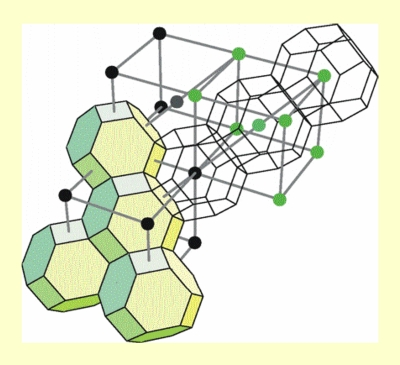
\includegraphics[width=0.4\textwidth]{figures/2_1wignerseitz.jpg}
    \caption{Wigner-Seitz Zelle}
    \label{}
\end{figure}
\begin{itemize}
    \item primitive EZ, die die volle Symmetrie des Gitters wiederspiegelt
    \item enthält den Teil des Raumes um einen Gitterpunkt, der diesem näher ist als den übrigen Gitterpunkten
    \item Konstruktionsvorschrift:
          \begin{itemize}
              \item[1.] Verbindungslinien von Gitterpunkt zu Nachbarn (Folie 4, grün gestrichelt)
              \item[2.] Mittelsenkrechte (Mittelebene, 3D) auf diesen Linien
              \item[3.] Wigner-Seitz-Zelle ist die kleinste eingeschlossene Fläche/Volumen
          \end{itemize}
\end{itemize}
\begin{figure}[H]
    \centering
    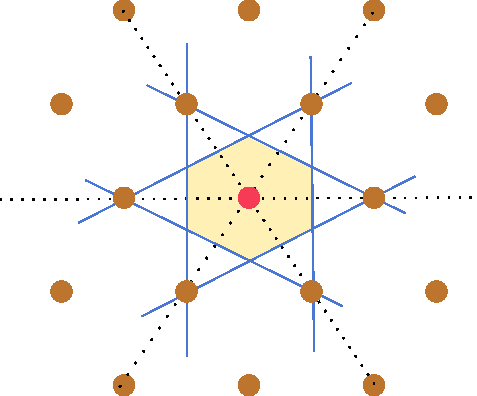
\includegraphics{figures/2_1Gitter.pdf}
    \caption{Beispiel}
    \label{}
\end{figure}
\paragraph{Symmetrien:}
\begin{itemize}
    \item[(a)] Translationssymmetrie:\\
          Kristallgitter ist invariant unter Transformation mit Translationsvektor $\textbf{T} = n_1 \textbf{a}_1 + n_2 \textbf{a}_2 +n_3 \textbf{a}_3$ ($n_1$, $n_2$, $n_3$ ganzzahlig)
          \begin{itemize}
              \item[$\rightarrow$] Für jeden Punkt \textbf{r} mit Umgebung $\mathcal{U} (\textbf{r})$: identische Umgebung am Ort \textbf{r} + \textbf{T}, also $\mathcal{U} (\textbf{r} + \textbf{T}) = \mathcal{U} (\textbf{r})$
              \item[$\rightarrow$] Durch Translation der primitiven EZ lässt sich der Raum lückenlos und ohne Überlapp auffüllen.
              \item[$\rightarrow$] Durch Translation um die primitiven GV lässt sich jeder Gitterpunkt erreichen.
          \end{itemize}
          {figure}\begin{figure}[H]
            \centering
            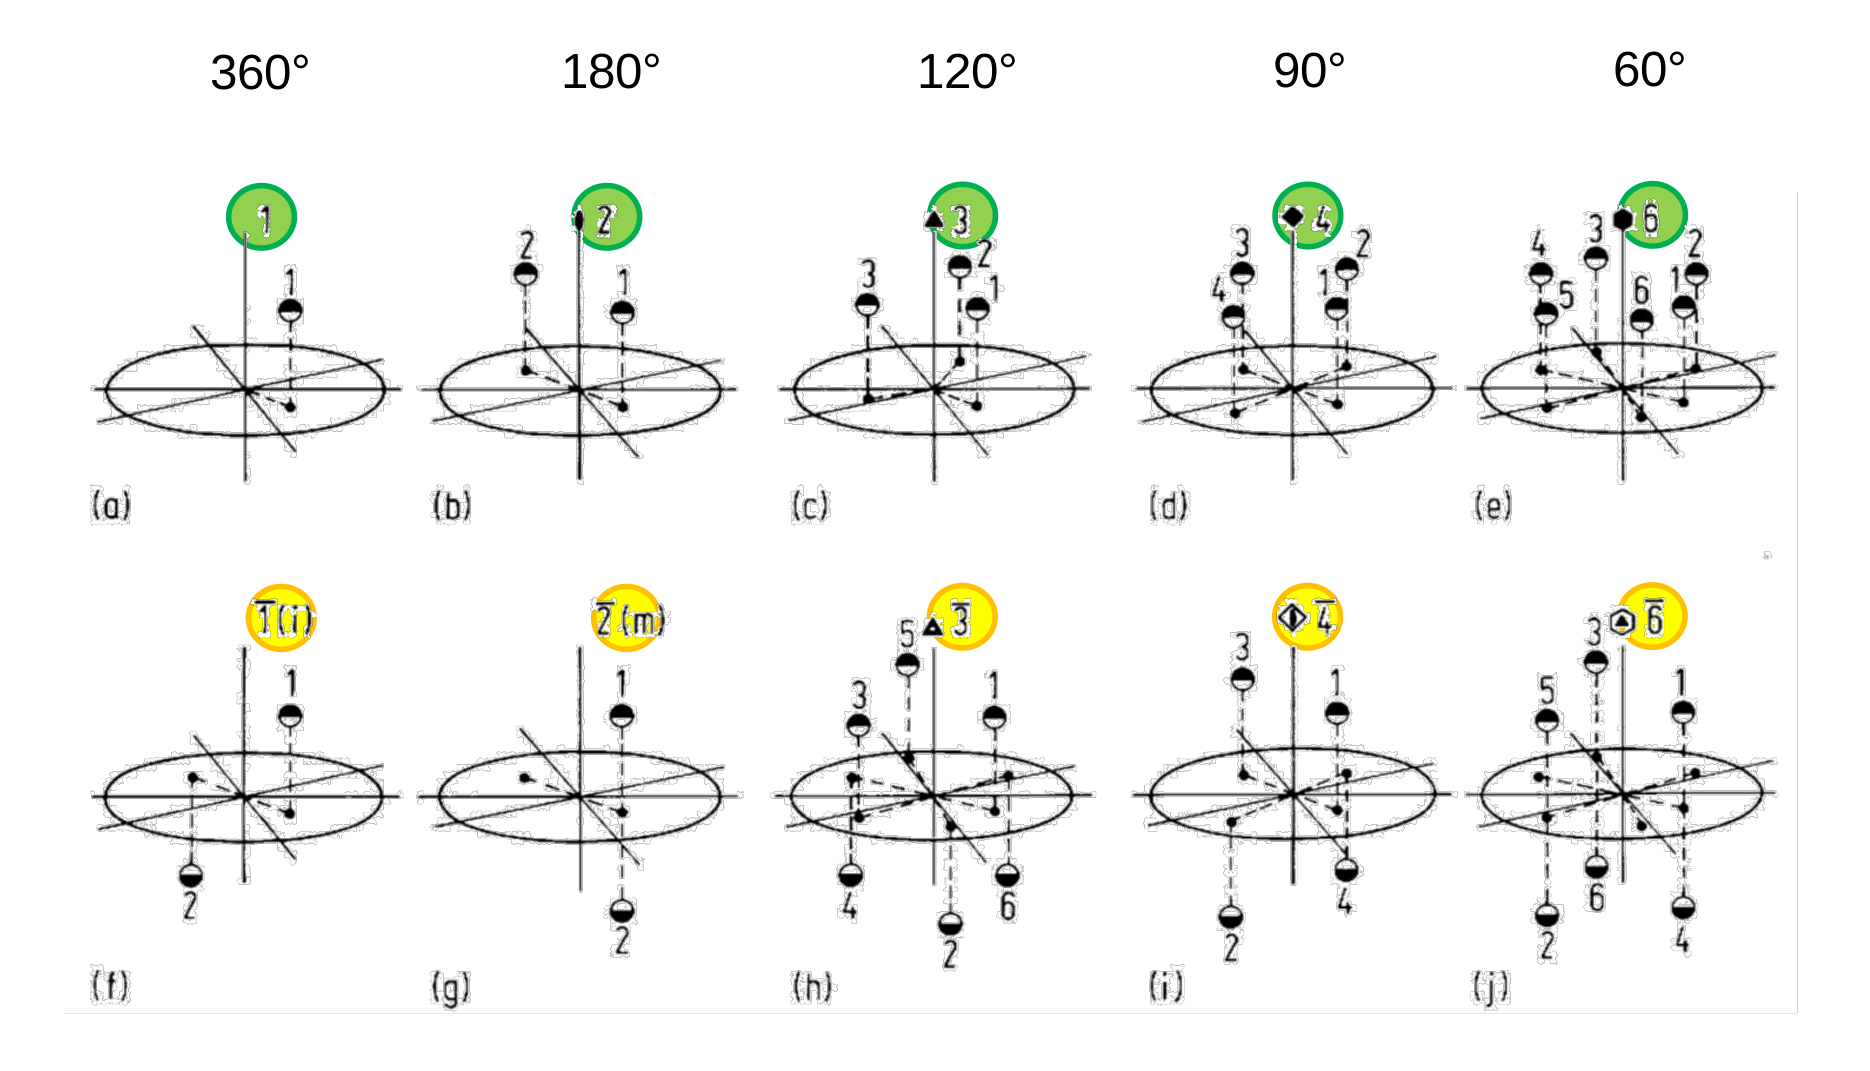
\includegraphics[width=\textwidth]{figures/2_1Symmetrie}
            \caption{Symmetrieoperationen der Punktgruppe}
            \label{}
        \end{figure}
    \item[(b)] Punktsymmetrie-Operationen:\\
          Unter Punktsymmetrie-Operationen bleibt mindestens 1 Punkt im Raum unverändert
          \begin{itemize}
              \item[(i)] \textbf{Drehung um eine Drehachse:}\\
                    Drehung, unter denen das Gitter invariant ist:
                    \begin{table}[H]
                        \centering
                        \begin{tabular}{l|lllll}
                            Winkel in rad             & $2 \pi$ & $\frac{2\pi}{2}$ & $\frac{2\pi}{3}$ & $\frac{2\pi}{4}$ & $\frac{2\pi}{6}$ \\\hline
                            Zähligkeit der Drehachsen & 1       & 2                & 3                & 4                & 6
                        \end{tabular}
                    \end{table}
                    \textbf{NB:} Es gibt kein Kristallgitter mit Zähligkeit $>6$. Es gibt kein Kristallgitter mit 5-zähliger Symmetrie. Diese ist kompatibel mit Translationssymmetrie. Quasikristalle haben 5-zählige Symmetrie, sind aber nicht periodisch.
              \item[(ii)] \textbf{Spiegelung:} $x  \rightarrow  -x$, $y  \rightarrow y$, $z  \rightarrow  z$; Symbol: m
              \item[(iii)] \textbf{Inversion:} $x  \rightarrow  -x$, $y  \rightarrow -y$, $z  \rightarrow  -z$; Symbol: i oder 1\\
                    (Rotation um $\frac{2 \pi}{2} +$ Spiegelung an Ebene $\bot$ Drehachse)
              \item[(iv)] \textbf{Drehinversion} Drehung mit Zählgebiet 1,2,3,4,6,+ Inversionen; Symbol: z.B. $\overline{3} \rightsquigarrow $ 10 Symmetrieoperatoren der Punktgruppe.
          \end{itemize}
    \item[(c)] Klassifikation von Kristallgittern: \\
        Schema zur Einordnung von Kristallgittern nach ihren Symmetrieeigenschaften.
        \begin{itemize}
              \item[(I)] \textbf{Kristallsysteme}: \\ Gitterpunktgruppen, Symmetrie bzgl. Punktsymmetrie-Operationen.\\
              In 3D gibt es 7 Kristallsysteme:
              \begin{table}[H]
                \centering
                \begin{tabular}{l|llll}
                  Kristallsystem & Gitterkonstanten & Winkel & Zähligkeit & Anzahl\\\hline
                  triklin & $a_1 \neq a_2 \neq a_3$ & $\alpha \neq \beta \neq \gamma$ & 1 &  \\
                  monoklin & $a_1 \neq a_2 \neq a_3$ & $\alpha = \beta = 90^{\circ} \neq \gamma$ & 2 &  \\
                  orthorhombisch & $a_1 \neq a_2 \neq a_3$ & $\alpha = \beta = \gamma = 90^{\circ}$ & 2 &  \\
                  tetragonal & $a_1 = a_2 \neq a_3$ & $\alpha = \beta = \gamma = 90^{\circ}$ & 4 &  \\
                  hexagonal & $a_1 = a_2 \neq a_3$ & $\alpha = \beta = 90^{\circ}$; $\gamma = 120^{\circ}$ & 6 &  \\
                  trigonal & $a_1 = a_2 = a_3$ & $\alpha = \beta  = \gamma \neq 90^{\circ}$ & 3 &  \\
                  kubisch & $a_1 = a_2 = a_3$ & $\alpha = \beta = \gamma = 90^{\circ}$ & 3 &  \\
                \end{tabular}
            \end{table}
            Im FK treten häufig kubische oder hexagonale Kristallsysteme auf. Grund: Atome (Bausteine) sind $\approx$ kugelsymmetrisch, daher Hochsymmetrie bevorzugt.
            \item[(II)] \textbf{Bravais-Gitter:}\\
            Gitter-Raumgruppe, Symmetrie bzgl. Punkt- und Translationsoperationen.
            \begin{figure}[H]
                \centering
                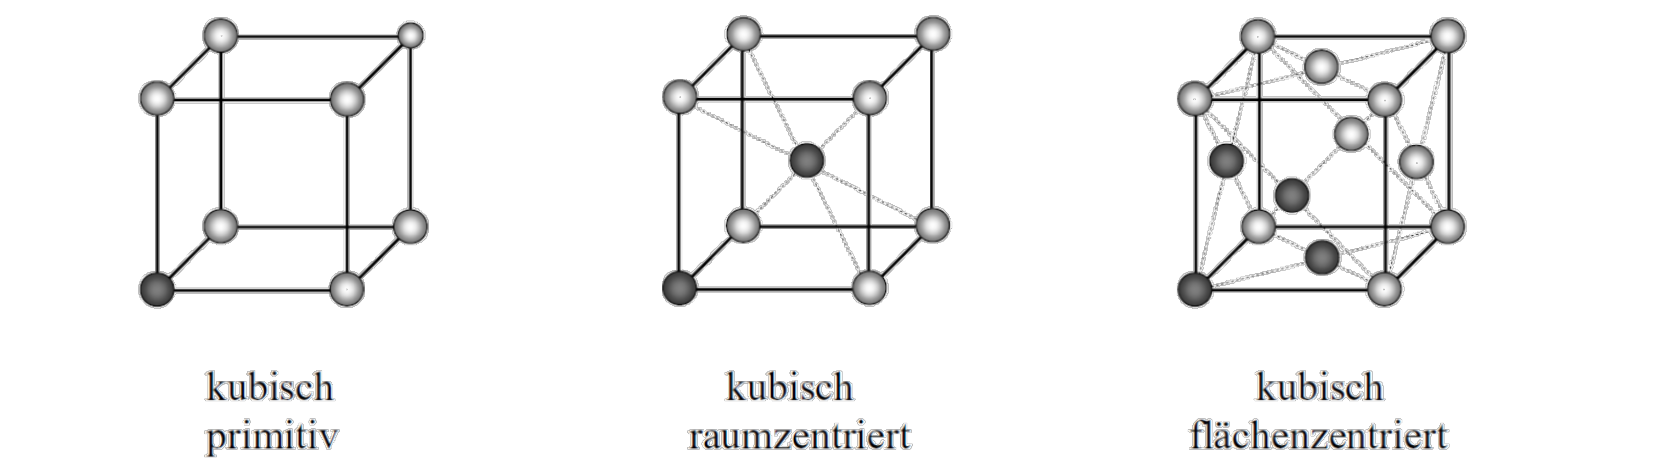
\includegraphics[width=0.7\textwidth]{figures/2_1KubischGitter}
                \caption{Beispiele für Bravais-Gitter}
            \end{figure}
            3D: 14 Bravais-Gitter
            \begin{itemize}
                \item So konstruiert, dass sie Symmetrie des Gitters widerspiegeln, dass sie also die höchste Zahl an Punktsymmetrie-Operationen enthalten.
                \item Nur 7 Bravais-Gitter haben primitive Elementarzelle.
            \end{itemize}
        \end{itemize}
\end{itemize}
\subsection{Einfluß der Basis} \label{kap:2_2}
Bisher: Nur Gitter. In 3D: 7 Kristallgitter (Gitter-Punktgruppen)\\
14 Bravisgitter (Gitter-Punktgruppen)\\
\begin{itemize}
    \item Beschreibung der Symmetrie Atomm $\rightarrow$ keine Änderung
    \item i.A. Basis komplizierter:\\
    z.B kubisch primitives Gitter:
    \begin{figure}[H]
        \centering
        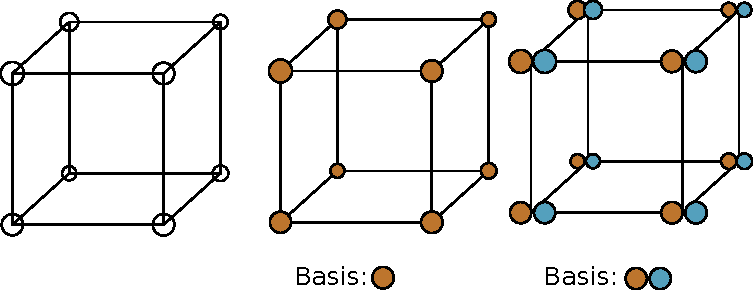
\includegraphics{figures/2_2Cubes.pdf}
        \caption{}
        \label{}
    \end{figure}
\end{itemize}
Analyse der Symmetrie des Kristalls (Gitter + Basis)\\
32 Kristallklassen (Punktgruppen)\\
230 Kristallophysische Raumgruppen (Raumgruppen)\\
\subsection{Beispiele einfacher Kristallstrukturen}
\label{kap:2_3}
Hier: Kristallstrukturen, die besonders häufig auftreten.
\begin{itemize}
    \item Chemische Elemente:\\
    kubisch flächenzentriert (fcc): 21\\
    kubisch raumzentriert (bcc): 16\\
    hexagonal (hcp: hexagonal close packed): 33\\
    , aber: kubisch primitiv (sc = simple cubic): 1 ($\alpha$-Po)
    \item Weitere häufige Strukturen
    \begin{itemize}
        \item Diamant
        \item Zinkblende
        \item Kochsalz
        \item Cäsiumchlorid
    \end{itemize}
\end{itemize}
\begin{figure}[H]
    \centering
    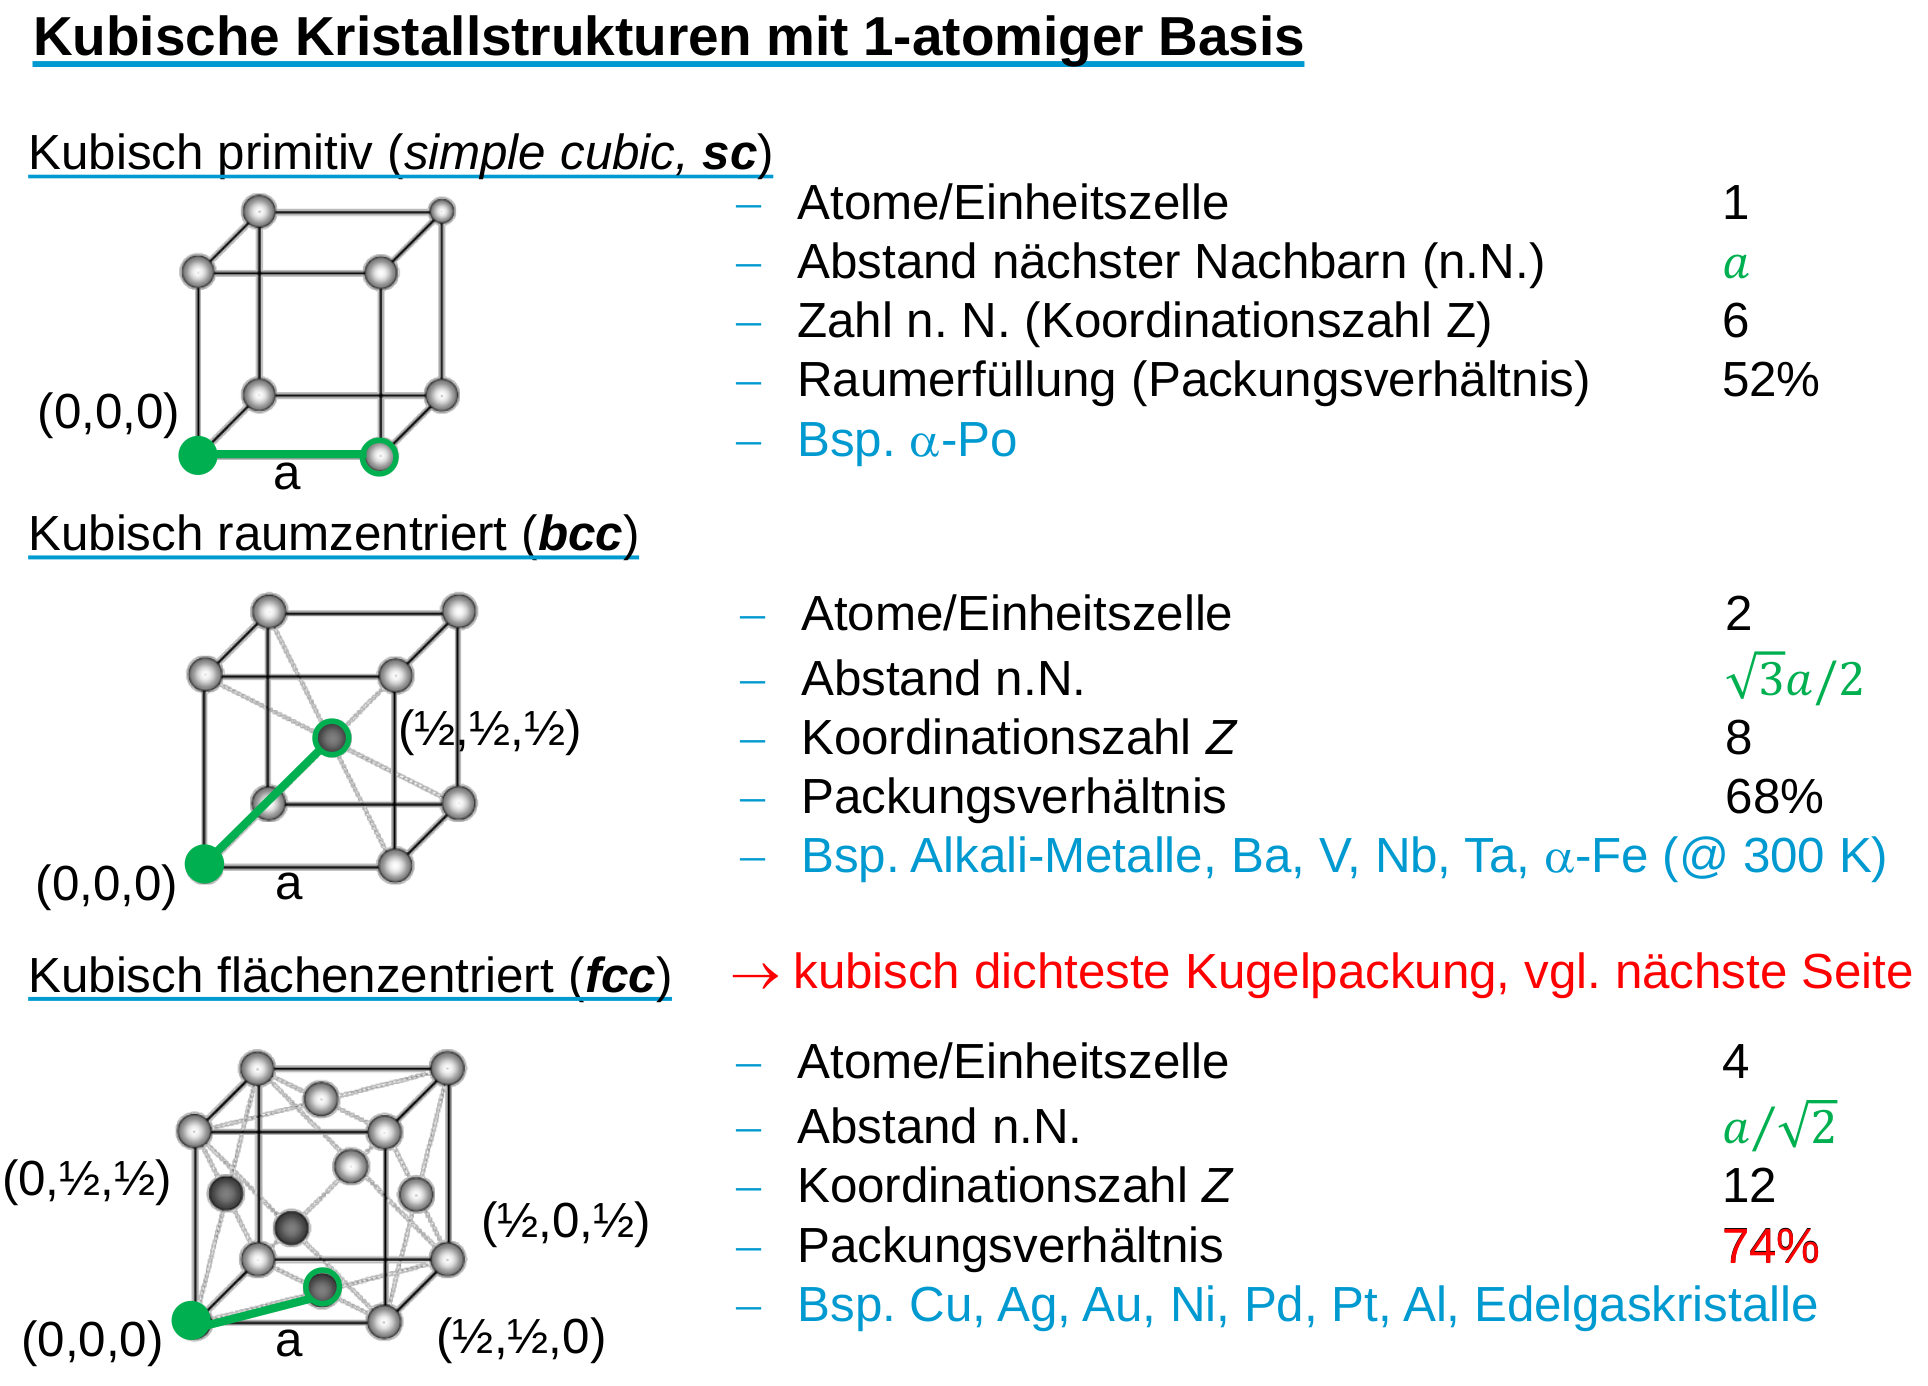
\includegraphics[width = \textwidth]{figures/2_2Kristallstrukturen1A.png}
    \caption{Vorlsungsfolie}
    \label{}
\end{figure}
\subsection{Indizierung von Kristallebenen und Richtungen}
\label{kap:2_4}
\textbf{Def:} Kristallebene (Gitterebene, Netzebene)
\begin{itemize}
    \item Ebene im Kristall, die durch Gitterpunkte aufgespannt wird.
    \item Tranlationsinvarianz des Kristalls: immer $\infty$ viele äquivalente Ebenen parallel zu jeder Kristallebene liegten.
    \item Festlegung durch Angabe der Durchstoßpunkte der Gitterachsen \textbf{a,b,c}
    \begin{figure}[H]
        \centering
        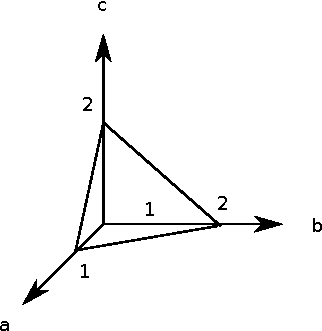
\includegraphics{figures/2_4dreieck.pdf}
        \caption{}
        \label{}
    \end{figure}
    \item Millerschen Indizes: Bezeichnung von Kristallebenen. Bestimmungsverfahren:
    \begin{itemize}
        \item[(1)] Durchstoßpunkte in Einheiten der Gitterkonstante, z.B. 122
        \item[(2)] Kehrwert, z.B. $1, \frac{1}{2}, \frac{1}{2}$
        \item[(3)] Multiplikationen mit kleinstmöglichem Faktor, der ganze Zahlen liefert (hier: 2) führt auf Millersche Indizes hkl, z.B. 211
    \end{itemize}
    \begin{itemize}
        \item Sonderfälle:\\
        Kristallebene || Gittervektor $\rightarrow$ Schnittpunkt $\infty$, index 0
        \item Durchstoßpunkt auf negativer Achse: Notation $1$ oder $2$
    \end{itemize}
    \paragraph{Diskussion:}
    \begin{itemize}
        \item Miller Indizes hängen von der Wahl der Gittervektoren ab.
        \item (hkl) bezeichnet Schar von Ebenen, die parallel sind.
        \item [hkl] bezeichnet Vektor $h\cdot \textbf{a}_1 + k \cdot \textbf{a}_2 + l \cdot \textbf{a}_3$ (Kristallrichtung)\\
        In kubischen Kristallen steht [hkl] senkrecht auf (hkl)
        \item \{hkl\} Gesamtheit aller symmetriebedingt gleichwertigen Ebenenscharen.
        \item <hkl> Gesamtheit aller symmetriebedingt gleichwertigen Kristallrichtungen.\\
        z.B. kubisches Gitter:\\
        <100>: [100], [$\overline{1}$00], [010], [1$\overline{1}$0], [001], [00$\overline{1}$]\\
        <110>: [110], [$\overline{1}$10], [1$\overline{1}$0], [$\overline{1}$$\overline{1}$0], [101], [$\overline{1}$01], [10$\overline{1}$], [$\overline{1}$0$\overline{1}$], [011], [0$\overline{1}$1], [01$\overline{1}$], [0$\overline{1}$$\overline{1}$]
        \item hexagonale Gitter haben oft unintuitive Miller-Indizes\\
        \begin{figure}[H]
            \centering
            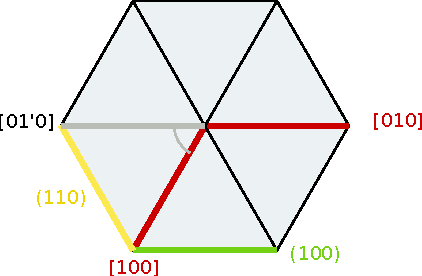
\includegraphics[]{figures/2_4Hexa.pdf}
            \caption{\{100\} enthält (100), aber nicht (1$\overline{1}$0)\\
            $\rightsquigarrow$ 4. Index $i = -(h+k)$: hkil also für obiges Beispiel {10$\overline{1}$0}}
            \label{}
        \end{figure}
	\end{itemize}
\end{itemize}
